\documentclass[12pt]{article}

\usepackage{sbc-template}

\usepackage{graphicx,url}

%\usepackage[brazil]{babel}   
\usepackage[latin1]{inputenc}  

\usepackage{amsmath}
\usepackage{amssymb} 
\usepackage{mathtools}

\usepackage{algorithm}
\usepackage{algpseudocode}

 
\newcommand{\Cfield}{\mathbb{C}}
\newcommand{\Rfield}{\mathbb{R}}

\newcommand{\norm}[1]{\left\lVert#1\right\rVert}

\sloppy

\title{Instructions for Authors of SBC Conferences\\ Papers and Abstracts}

\author{Luciana P. Nedel\inst{1}, Rafael H. Bordini\inst{2}, Fl�vio Rech
  Wagner\inst{1}, Jomi F. H�bner\inst{3} }


\address{Instituto de Inform�tica -- Universidade Federal do Rio Grande do Sul
  (UFRGS)\\
  Caixa Postal 15.064 -- 91.501-970 -- Porto Alegre -- RS -- Brazil
\nextinstitute
  Department of Computer Science -- University of Durham\\
  Durham, U.K.
\nextinstitute
  Departamento de Sistemas e Computa��o\\
  Universidade Regional de Blumenal (FURB) -- Blumenau, SC -- Brazil
  \email{\{nedel,flavio\}@inf.ufrgs.br, R.Bordini@durham.ac.uk,
  jomi@inf.furb.br}
}

\begin{document} 

\maketitle

\begin{abstract}
  This meta-paper describes the style to be used in articles and short papers
  for SBC conferences. For papers in English, you should add just an abstract
  while for the papers in Portuguese, we also ask for an abstract in
  Portuguese (``resumo''). In both cases, abstracts should not have more than
  10 lines and must be in the first page of the paper.
\end{abstract}
     
\section{Introduction}

Parallel computing is hard to define, but intuitively, it is a computation method 
that allows data to be distributed and processed simultaneously. In Flynn's taxonomy
\cite{pacheco:2011},
there are two types of parallel computer archictectures: 

\begin{enumerate}
\item Single Instruction, Multiple Data (SIMD); a processor that allows a chunk of
data to be loaded and a single instruction to be used to process it. Intel's SSE 
and Graphics Processing Units (GPU) are examples it. 

\item Multiple Instruction, Multiple Data (MIMD); a system consisting of
multiple independent processing units, executing asynchronously. Here are located 
all multicore Shared-memory systems and Distributed-memory systems.
\end{enumerate}

GPU was originally designed to renderize graphics in real time, however, researchers 
realized that GPU could be used for general purpose applications. OpenGL and DirectX 
were designed to access GPUs resources, both are specialized to produce graphics. 
These libraries were used by engineers and scientists in their specific problems, 
as a result, they had to convert their problem into a graphical domain.

NVIDIA noticed a new demand for their products and created an API called CUDA with 
the goal enable the use of GPUs in general purpose situation.

CUDA consists of kernels, which are functions that run in a GPU in a parallel fashion. 
A kernel is organized into a set of blocks. A block is a set of threads that cooperate 
between themselves \cite{patterson:2007}.  

A kernel accesses data from GPU's memory. Its memory is divided between global memory, 
a memory that all threads can access; a local memory, a memory that is private to a thread; 
and shared memory, a  low-latency memory that is shared between all threads in the same block
\cite{patterson:2007}. 



The Bondary Elements Method (BEM) is a computational method of solving linear
partial differentials equations that have been formulated as integral equations.
This is used in many areas of engineering, but this article presents a Graphical
Unit Processor (GPU) accelerated implementation of BEM with the purpose of
analysing waves propagation on the ground and it's effects on nearby structures.

Given a sequential implementation of such method by \cite{carrion:02}, the main objectives
of this project includes the creation of automated tests to check if the modified 
program results are numerically compatible with the original version; somewhat 
modernize the legacy code, which was written in Fortran 77; optimize the code, 
removing repeated unnecessary calculations and managing a better usage of the 
Central Processing Unit (CPU) resources; 
identify the most time-consuming subroutines and paralellize them.

This project was supported by CAPES and \textbf{BLABLABLABLABLABLA} (n�o sei muito bem
o que colocar aqui)

\section{Norms}

In order to check if the final result obtained by the parallel program is numerically 
compatible with the original, the concept of vector and matrix norms are necessary. 
Let $x \in \Cfield^n$ and $A \in \Cfield^{m \times n}$. \cite{watkins:2004} defines a 
vector $\infty$-norm, matrix $\infty$-norm and matrix 1-norm as:
\begin{equation}
	\norm{x}_{\infty} = \max\limits_{1 \leq k \leq n} |x_k| \qquad 
	\norm{A}_{\infty} = \max\limits_{1 \leq i \leq m} \sum_{j=1}^{n} |a_{ij}| \quad
	\norm{A}_{   1  } = \max\limits_{1 \leq j \leq n} \sum_{i=1}^{m} |a_{ij}| \quad
\end{equation}

All vector norms have the propierty that $\norm{x} = 0$ if and only if $x = 0$, and
the same result asserts for matrix norms. Let $f$ and $g$ be two numerical 
algorithms that solves the same problem, but in a different fashion. 
Let now $y_f$ be the result computed by $f$ and $y_g$ be the result computed by
$g$. The \textit{error} between those two values can be measured computing
$\norm{y_f - y_g}$.

%Let now $\hat{x} \in \Cfield^n$
%be a value that should have been $x$, but contains errors due to whatever
%reasons. One can measure \textit{how far} $\hat{x}$ is from $x$ by computing
%$\norm{x - \hat{x}}$. If the vector $\infty$-norm is used, then the result yielded
%is the maximum difference between a single entry of the vector. If the matrix
%$\infty$-norm is used, then the result is the biggest sum of errors of a matrix
%row. The matrix 1-norm yields the biggest sum of erros of a matrix column.

\section{Parallelization Technique}

A parallel implementation of BEM began by analyzing and modifying a sequential code 
provided by Carrion. Gprof \cite{binutils}, a profiling tool by GNU, showed that the most time-consuming 
routine was Nonsingd, a subroutine designed to solve small parts of the nonsingular dynamic 
problem. Since most calls to Nonsingd were from Ghmatecd, most of the parallelization effort 
was focused on that last routine.

\subsection{Ghmatecd Parallelization}
Ghmatecd works in the following way: It assembles two complex matrices H and G by computing 
smaller $3 \times 3$ matrices returned by Nonsingd and Sigmaec. Let $n$ be the number of 
\textbf{ELEMENTOS DE MALHA} and $m$ \textbf{ELEMENTOS DE CONTORNO} The following pseudocode 
illustrates how Ghmatecd works:

\begin{algorithm}
\caption{Creates $H, G \in \Cfield^{(3m)\times(3n)}$}\label{euclid}
\begin{algorithmic}[1]
	\Procedure{Ghmatecd}{}
		\For{$j := 1, n$} 
			\For{$i := 1, m$}
				\State{$ii := 3(i-1) + 1;     jj := 3(j-1) + 1$}
				\If{$i == j$}
					\State{$Gelement, Helement \leftarrow \text{Sigmaec}(i, j)$}\Comment{two $3\times3$ complex matrices}					
				\Else
					\State{$Gelement, Helement \leftarrow \text{Nonsingd}(i, j)$}	
				\EndIf
				\State{$G[ii:ii+2][jj:jj+2] \leftarrow Gelement$}
				\State{$H[ii:ii+2][jj:jj+2] \leftarrow Helement$}
			\EndFor
	 \EndFor
	\EndProcedure
\end{algorithmic}
\end{algorithm}

There is no interdependency between iteractions, so the two nested loop in the algorithm can be computed in parallel, 
hence, both matrices $H$ and $G$ can be built in a parallel fashion. If the number of processors is small, 
then parallelizing the two nested loops in line computing that nested loop in parallel is enough because even for small instances of the problem, 
$n \times m$ will be bigger than the number of processors.
By other hand, GPUs have greater parallel capability than CPUs, and the above strategy alone would generate a waste of 
computational resources. A careful analysis of both Nonsingd and Sigmaec codes concluded that a certain degree of 
parallelism can be explored in those procedures in order to take advantage of GPUs. Both procedures have a two nested 
loop that generates various 3x3 matrices. Before returning, those procedures do a reduction of these matrices. 
It should be highlighted that Sigmaec and Nonsingd are almost identical, so both can be merged into a single routine 
with a special logic to check if it needs to solve the singular or the nonsingular problem. Let $g$ be the number
of Gauss quadrature points. If this new procedure is unrolled in Ghmatecd, then there would be:

\begin{algorithm}
\caption{Creates $H, G \in \Cfield^{(3m)\times(3n)}$}\label{euclid}
\begin{algorithmic}[1]
	\Procedure{Ghmatecd}{}
		\For{$j := 1, n$} 
			\For{$i := 1, m$}
				\State{$ii := 3(i-1) + 1;     jj := 3(j-1) + 1$}
				\State{Allocate \textit{Hbuffer} and \textit{Gbuffer}, buffer of matrices $3 \times 3$ of size $g \times g$}
				\For{$y := 1, g$}
					\For{$x := 1, g$}
						\State{\textit{params} $\leftarrow$ ComputeParameters$(i, j, x, y)$}
						\State{$\textit{Hbuffer}(x, y) \leftarrow \text{GenerateMatrixH}(x, y, params)$}
						\State{$\textit{Gbuffer}(x, y) \leftarrow \text{GenerateMatrixG}(x, y, params)$}
						\If{$i == j$}
							\State{$\text{SpecialLogicForSingularCase}(\textit{Hbuffer}(x, y), \textit{Gbuffer}(x, y))$}
						\EndIf
					\EndFor
				\EndFor
				\State{$Gelement \leftarrow \text{SumAllMatricesInBuffer}(\textit{Gbuffer})$} 
				\State{$Helement \leftarrow \text{SumAllMatricesInBuffer}(\textit{Hbuffer})$}
				\State{$G[ii:ii+2][jj:jj+2] \leftarrow Gelement$}
				\State{$H[ii:ii+2][jj:jj+2] \leftarrow Helement$}
			\EndFor
	 \EndFor
	\EndProcedure
\end{algorithmic}
\end{algorithm}

The algorithm2 can be implemented in CUDA kernel in the following way: Inside a block, create $g \times g$ threads to 
compute in parallel the two nested loop in lines 6 to 7, allocating \textit{Hbuffer} and \textit{Gbuffer} in shared 
memory. Since these buffers contain matrices of size $3 \times 3$, $9$ of these $g \times g$ threads can be used to 
sum all matrices. Notice that $g \geq 3$ is necessary for that condition, and that $g$ is also upper-bounded by the 
amount of shared memory available in the GPU. Launching $m \times n$ blocks to cover the two nested loops in lines
2 to 3 will generate the entire $H$ and $G$.

\subsection{Ghmatece Parallelization}

Ghmatece is a routine designed to create two real matrices H and G associated with the static problem, and it 
is very similar to Ghmatecd. That routine can be implemented in CUDA in almost the same way as Ghmatecd, but 
caution is needed because the singular case has a lot of ifs that can cause branch divergence, thus affecting 
performance in a negative way. 
Since the singular case is dimensionally smaller than the non-singular case, it can be computed in the CPU 
and the result merged with the non-singular case calculated in the GPU. 

\section{General Information}

All full papers and posters (short papers) submitted to some SBC conference,
including any supporting documents, should be written in English or in
Portuguese. The format paper should be A4 with single column, 3.5 cm for upper
margin, 2.5 cm for bottom margin and 3.0 cm for lateral margins, without
headers or footers. The main font must be Times, 12 point nominal size, with 6
points of space before each paragraph. Page numbers must be suppressed.

Full papers must respect the page limits defined by the conference.
Conferences that publish just abstracts ask for \textbf{one}-page texts.

\section{First Page} \label{sec:firstpage}

The first page must display the paper title, the name and address of the
authors, the abstract in English and ``resumo'' in Portuguese (``resumos'' are
required only for papers written in Portuguese). The title must be centered
over the whole page, in 16 point boldface font and with 12 points of space
before itself. Author names must be centered in 12 point font, bold, all of
them disposed in the same line, separated by commas and with 12 points of
space after the title. Addresses must be centered in 12 point font, also with
12 points of space after the authors' names. E-mail addresses should be
written using font Courier New, 10 point nominal size, with 6 points of space
before and 6 points of space after.

The abstract and ``resumo'' (if is the case) must be in 12 point Times font,
indented 0.8cm on both sides. The word \textbf{Abstract} and \textbf{Resumo},
should be written in boldface and must precede the text.

\section{CD-ROMs and Printed Proceedings}

In some conferences, the papers are published on CD-ROM while only the
abstract is published in the printed Proceedings. In this case, authors are
invited to prepare two final versions of the paper. One, complete, to be
published on the CD and the other, containing only the first page, with
abstract and ``resumo'' (for papers in Portuguese).

\section{Sections and Paragraphs}

Section titles must be in boldface, 13pt, flush left. There should be an extra
12 pt of space before each title. Section numbering is optional. The first
paragraph of each section should not be indented, while the first lines of
subsequent paragraphs should be indented by 1.27 cm.

\subsection{Subsections}

The subsection titles must be in boldface, 12pt, flush left.

\section{Figures and Captions}\label{sec:figs}


Figure and table captions should be centered if less than one line
(Figure~\ref{fig:exampleFig1}), otherwise justified and indented by 0.8cm on
both margins, as shown in Figure~\ref{fig:exampleFig2}. The caption font must
be Helvetica, 10 point, boldface, with 6 points of space before and after each
caption.

\begin{figure}[ht]
\centering
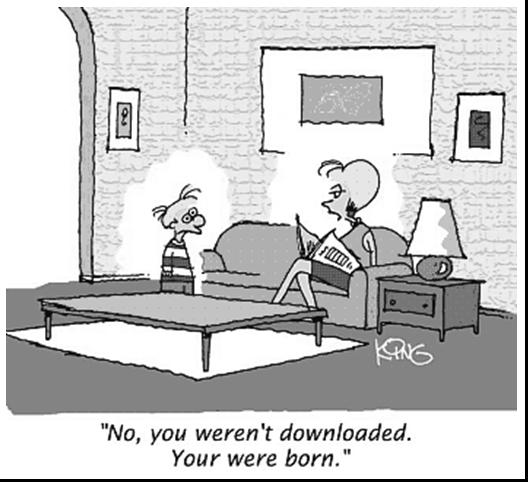
\includegraphics[width=.5\textwidth]{fig1.jpg}
\caption{A typical figure}
\label{fig:exampleFig1}
\end{figure}

\begin{figure}[ht]
\centering
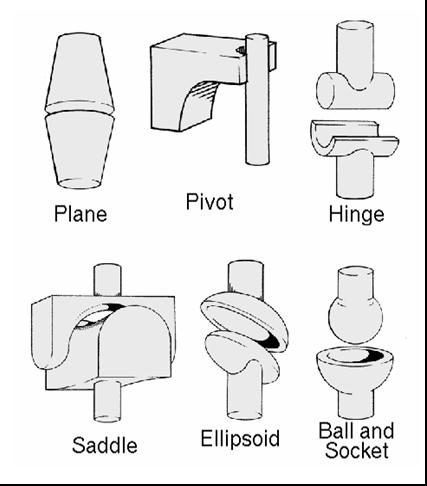
\includegraphics[width=.3\textwidth]{fig2.jpg}
\caption{This figure is an example of a figure caption taking more than one
  line and justified considering margins mentioned in Section~\ref{sec:figs}.}
\label{fig:exampleFig2}
\end{figure}

In tables, try to avoid the use of colored or shaded backgrounds, and avoid
thick, doubled, or unnecessary framing lines. When reporting empirical data,
do not use more decimal digits than warranted by their precision and
reproducibility. Table caption must be placed before the table (see Table 1)
and the font used must also be Helvetica, 10 point, boldface, with 6 points of
space before and after each caption.

\begin{table}[ht]
\centering
\caption{Variables to be considered on the evaluation of interaction
  techniques}
\label{tab:exTable1}
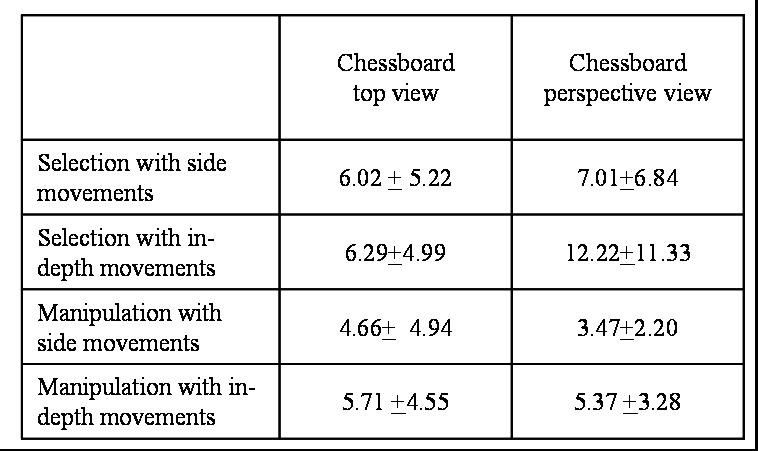
\includegraphics[width=.7\textwidth]{table.jpg}
\end{table}

\section{Images}

All images and illustrations should be in black-and-white, or gray tones,
excepting for the papers that will be electronically available (on CD-ROMs,
internet, etc.). The image resolution on paper should be about 600 dpi for
black-and-white images, and 150-300 dpi for grayscale images.  Do not include
images with excessive resolution, as they may take hours to print, without any
visible difference in the result. 

\section{References}

Bibliographic references must be unambiguous and uniform.  We recommend giving
the author names references in brackets, e.g. \cite{knuth:84},
\cite{boulic:91}, and \cite{smith:99}.

The references must be listed using 12 point font size, with 6 points of space
before each reference. The first line of each reference should not be
indented, while the subsequent should be indented by 0.5 cm.

\bibliographystyle{sbc}
\bibliography{sbc-template}

\end{document}
